\documentclass[a4paper, 11pt]{article}
\usepackage{geometry}
\geometry{letterpaper, margin=1in}
\usepackage{amsmath}
\usepackage{amssymb}  
\usepackage{amsthm}
\usepackage{ulem} 
\usepackage{graphicx}
\graphicspath{ {images/} }

\begin{document}
%Header-Make sure you update this information!!!!
\noindent
\large\textbf{Bessel Beam Intensity Derivation} \hfill \textbf{John Waczak} \\

First we will use the monochromatic plane wave to derive a general equation for light intensity. We will then use the Bessel beam condition in this equation to produce a formula for the intensity cross section in the plane perpendicular the the wavevector $\vec{k}$ (the direction of propagation). \\ 

Recall for a monochromatic plane wave, we can write: 
	\begin{align*}
		\mathbf{E} &= \mathbf{E}_0e^{i(\vec{k}\cdot\vec{r}-\omega t)}\\
		\mathbf{B} &= \mathbf{B}_0e^{i(\vec{k}\cdot\vec{r}-\omega t)} \\
		\text{with} \quad \mathbf{E} &\times \mathbf{B} = \vec{k} 
	\end{align*}
Now if we apply these equations to Faraday's law we have that: 
	\begin{align*}
		\nabla \times \mathbf{E} &= -\partial_t\mathbf{B} \\ 
		\nabla \times \mathbf{E}_0e^{i(\vec{k}\cdot\vec{r}-\omega t)} &= -\partial_t \mathbf{B}_0e^{i(\vec{k}\cdot\vec{r}-\omega t)} \\ 
		i\vec{k}\times \mathbf{E}_0e^{i(\vec{k}\cdot\vec{r}-\omega t)} &= i\omega \mathbf{B}_0e^{i(\vec{k}\cdot\vec{r}-\omega t)} \\ 
		(\vec{k}\times \mathbf{E}_0)ie^{i(\vec{k}\cdot\vec{r}-\omega t)} &=i\omega \mathbf{B}_0e^{i(\vec{k}\cdot\vec{r}-\omega t)} \\ 
		ikE_0\hat{\mathbf{B}}_0 &= i\omega B_0 \hat{\mathbf{B}}_0 \\ 
		\Rightarrow kE_0 &= \omega B_0 \\ 
		B_0 &= \frac{k}{\omega}E_0 = \frac{1}{c}E_0
	\end{align*}
Thus we have found a relationship between the magnitudes of the electric and magnetic fields. Using this relationship, we can greatly simplify our calculation of the Poynting vector. In order to do this though, we must first take the real part of our complex plane waves because \textbf{E} and \textbf{B} are real physical fields. 
	\begin{align*}
		|Re[\mathbf{E}]| &= E_0\cos(\vec{k}\cdot\vec{r}-\omega t) \\ 
		|Re[\mathbf{B}]| &= B_0\cos(\vec{k}\cdot\vec{r}-\omega t) \\ 
		\vec{S} &= \frac{1}{\mu_0}\mathbf{E} \times \mathbf{B} \\ 		
		&= \frac{1}{\mu_0}EB\vec{k} \\ 
		&= \frac{1}{\mu_0}E_0\cos(\vec{k}\cdot\vec{r}-\omega t)B_0\cos(\vec{k}\cdot\vec{r}-\omega t)\vec{k} \\ 
		&= \frac{1}{\mu_0}E_0B_0\cos^2(\vec{k}\cdot\vec{r}-\omega t)\vec{k} \\
		&= \frac{1}{\mu_0}E_0\frac{1}{c}E_0\cos^2(\vec{k}\cdot\vec{r}-\omega t)\vec{k} \\
		\frac{1}{\mu_0c} &= \frac{\epsilon_0}{\mu_0}=\epsilon_0c \\ 
		\Rightarrow \vec{S} &= \epsilon_0cE_0^2\cos^2(\vec{k}\cdot\vec{r}-\omega t)\vec{k}  
	\end{align*}
Now, because most measurements will consist of many full periods, we will consider the time averaged Poynting vector: 
	\begin{align*}
		\text{Recall} \quad \sin^2(\theta)+\cos^2(\theta) &=1 \\ 
		\text{thus over one period} \quad \langle \cos^2(\theta)\rangle &= \frac{1}{2} \\
		\Rightarrow \langle S \rangle &= \frac{1}{2}\epsilon_0 cE_0^2 \equiv I 
	\end{align*}	
Now we have that for an ideal Bessel beam, the magnitude of the electric field is described by: 
	\begin{equation*}
		E(r,\phi,z) = A_0J_\ell(k_r r)e^{i\ell\phi}e^{i(k_z z-\omega t)}
	\end{equation*}
where we are using the cylindrical coordinates in the xy plane $r,\phi,z$ and $J_\ell$ is a Bessel function of order $\ell$. Regardless of what direction this points, we can calculate the Poynting vector, and therefore the intensity, by simply taking the real part of this equation. 
	\begin{align*}
		Re[E] 	&= A_0J_\ell(k_r r)\cos(\ell\phi + k_zz-\omega t)\\
		\vec{S} &= \epsilon_0cA_0^2J_\ell^2(k_r r)\cos^2(\ell\phi + k_zz-\omega t)\vec{k} \\
		\text{thus} \quad \langle S \rangle &= \frac{1}{2}\epsilon_0cA_0^2J_\ell^2(k_r r)
	\end{align*}
If we graph a cross section of this intensity function (i.e. fixed value of z) we see that the beam consists of a series of annuli whose width are determined by the values of $k_r$, the radial component of the wavevector. The following figure illustrates I for a fixed value of $z=0$ and with other constants set arbitrarily to 1: 
	\begin{center}
		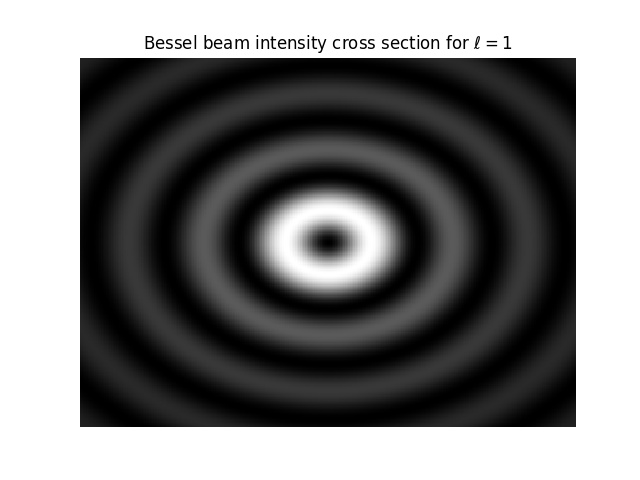
\includegraphics[scale=0.5]{intensityProfile}
	\end{center}
The only thing that remains is to verify that our Poynting vector equation holds for the bessel beam solution as it is not exactly the same as the monochromatic plane wave. 
\end{document}







































